\documentclass{article}
\usepackage[utf8]{inputenc}
\usepackage{graphicx}

\title{FPGA Example Design: Xilinx Zynq Board}
\author{JITX Team}
\date{\today}

\begin{document}

\maketitle

\section{Project Goals and Future Prospects}

\subsection{Primary Objectives}
\begin{itemize}
    \item Develop an FPGA design of moderate complexity using JITX, serving as a comprehensive overview of the tool's capabilities.
    \item Utilize this design as a stress test to identify and resolve bugs in the JITX toolchain, while ensuring adequate performance.
    \item Create a compelling marketing asset: A Zynq-based board represents a significant engineering challenge. Successfully implementing this design demonstrates JITX's ability to handle complex projects, appealing to professionals already working with the Zynq platform and those engaged in projects of similar complexity.
\end{itemize}

\subsection{Future Enhancements}
\begin{itemize}
    \item Refactor the codebase to improve reusability and parameterization, with the ultimate goal of integrating it into the JSL library.
    \item Expand the design to interface with a VPX backplane, contingent upon the development of a VPX backplane generator. This addition would transform the project into a highly attractive example for specific industry players, such as Lockheed-Martin.
    \item Potential to evolve into a world-class VPX backplane solution, further enhancing JITX's market position in specialized, high-performance computing applications.
\end{itemize}

\section{Architecture}

Here's the key components of the design:
\begin{enumerate}
    \item Xilinx Zynq SoC
    \item DDR4 memory
    \item Flash memory for bring-up
    \item ADC input to the FPGA, fed from a Coax connector
    \item HDMI output
    \item USB 2.0 and JTAG interface for bring-up and debugging
\end{enumerate}

\begin{figure}
    \centering
    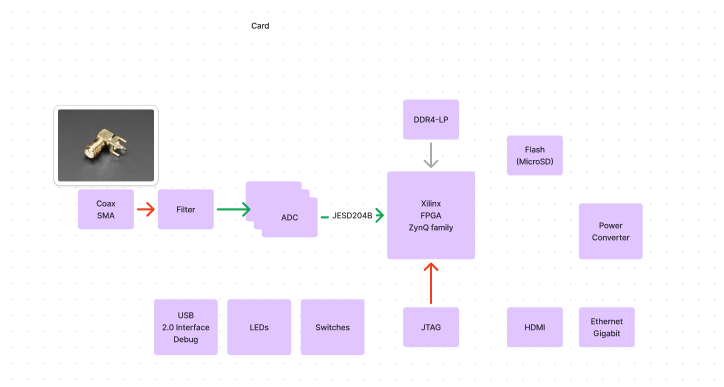
\includegraphics[width=0.8\textwidth]{../pics/block-diagram.png}
    \caption{Block diagram of the Zynq FPGA-based Design}
    \label{fig:fpga-block-diagram}
\end{figure}

\section{Part Selection}

\subsection{FPGA core}

Considering {\em XCZU1CG-1UBVA494I}:
\begin{itemize}
    \item Driven by need to support DDR4 memory. Lower-cost Zynq-7000 series only support up to DDR3.
    \item Lowest-cost Zynq Ultrascale+ part in stock on Digikey is XCZU1CG-1UBVA494I: \$292.52
    \item Dual core Arm Cortex-A53 (APU) + Dual core Arm Cortex-R5F (RPU)
    \item 81,900 Logic cells.
    \item 170 PS (Processing System) I/O, supporting 32-bit DDR4 only.
    \item 24 HD (High-Density) I/O. 58 HP (High-Performance) I/O.
\end{itemize}

\end{document}
